\chapter{Sprint 2 "Gestion de la tarification, souscription et consommation d'une API"}
	
\section*{Introduction}
Après avoir présenté dans le chapitre précédent le premier sprint, nous abordons, maintenant, le deuxième sprint. Celui-ci suit les mêmes étapes que le chapitre précédent, de la planification à la mise en œuvre, en mettant en exergue le backlog du sprint 2, ainsi que la spécification fonctionnelle, la conception, la revue du sprint et  pour conclure la rétrospective.


\section{ Extrait du backlog du sprint 2}
    Les thèmes du deuxième sprint sont : Gestion de la  tarification, souscription, test et consommation d'une API ainsi  que la gestion des comptes utilisateurs. \\
    Nous allons maintenant présenter un extrait du backlog du sprint à travers les users stories qui traitent la : Consommation d’une API et la souscription à une API  
    \begin{table}[H]
        \centering
        \caption{Extrait du backlog du sprint 2  "Consommation d'une API"}
        \label{tab:task_estimation_subscription}
    \begin{longtable}[c]{|p{0.25\linewidth}|p{0.25\linewidth}|p{0.25\linewidth}|p{0.15\linewidth}|}
        \hline
        \textbf{User story} & \textbf{Tâches} & \textbf{Sous-tâches} & \textbf{Estimation} \\
        \hline
        \endfirsthead
        \multicolumn{4}{c}%
        {{\bfseries \tablename\ \thetable{} -- suite de la page précédente}} \\
        \hline
        \textbf{User story} & \textbf{Tâches} & \textbf{Sous-tâches} & \textbf{Estimation} \\
        \hline
        \endhead
        \hline \multicolumn{4}{|r|}{{\bfseries Suite à la page suivante}} \\
        \hline
        \endfoot
        \hline
        \endlastfoot

        \multirow{8}{=}{En tant que développeur, je veux pouvoir consommer une API.}
            & Recherche & Documentation & 7\\
        \cline{2-4}
            & \multirow{2}{=}{Modélisation \& conception UML} & Réalisation du diagramme d’activités & 2h \\
        \cline{3-4}
            & & Réalisation du diagramme de séquence & 2h \\
        \cline{2-4}
            & \multirow{2}{=}{Préparation du backend} & Réalisation de la fonction post “consumeAPI” & 10h \\
        \cline{3-4}
            & & Test & 1h \\
        \hline
    \end{longtable}
    \end{table}

    \begin{table}[H]
        \centering
        \caption{Extrait du backlog du sprint 2  "Souscription à une API"}
        \label{tab:task_estimation_subscription}
        \begin{longtable}{|p{0.25\linewidth}|p{0.25\linewidth}|p{0.25\linewidth}|p{0.15\linewidth}|}
            \hline
            \textbf{User story} & \textbf{Tâches} & \textbf{Sous-tâches} & \textbf{Estimation} \\
            \hline
            \endfirsthead
            \multicolumn{4}{c}%
            {{\bfseries \tablename\ \thetable{} -- suite de la page précédente}} \\
            \hline
            \textbf{User story} & \textbf{Tâches} & \textbf{Sous-tâches} & \textbf{Estimation} \\
            \hline
            \endhead
            \hline \multicolumn{4}{|r|}{{\bfseries Suite à la page suivante}} \\
            \hline
            \endfoot
            \hline
            \endlastfoot
    
            \multirow{10}{=}{En tant que développeur, je veux pouvoir souscrire à une API pour accéder aux fonctionnalités qu'elle propose.}
                & Préparation de la Maquette & Réalisation de la maquette & 4h \\
            \cline{2-4}
                & Recherche & Documentation & 6h \\
            \cline{2-4}
                & \multirow{1}{=}{Modélisation \& conception UML} & Réalisation du diagramme d’activités & 2h \\
            \cline{2-4}
                & \multirow{2}{=}{Préparation du backend} & Réalisation de la fonction post "createSubscription” & 8h \\
            \cline{3-4}
                & & Test & 2h \\
            \cline{2-4}
                & \multirow{3}{=}{Préparation du frontend} & Modification de l’interface “API plans” & 4h \\
            \cline{3-4}
                & & Validation du formulaire & 1h \\
            \cline{3-4}
                & & Préparation du service “SubscriptionService” & 2h \\
            \cline{3-4}
                & & Préparation de la fonction “onsubmit” & 2h \\
            \cline{3-4}
                & & Test & 1h \\
            \hline
        \end{longtable}
    \end{table}

\section{Spécification fonctionnelle}
Dans cette partie nous allons présenter le diagramme de cas d'utilisation et un exemple de maquette.
  \subsection{Diagramme de cas d'utilisation}
  Dans notre diagramme de cas d'utilisation, nous incluons les nouveaux cas d'utilisation :
  \begin{itemize}
    \item  \textbf{Développeur}
    \begin{itemize}
        \item  Consulter les plans de tarification d'une API.
        \item Gérer mes souscriptions.
        \item Tester une API.
        \item Consommer une API.
        \item Gérer mon profil.
    \end{itemize} 
    \pagebreak

    \item  \textbf{Administrateur}
    \begin{itemize}
        \item Consulter les plans de tarification d'une API.
        \item Consommer une API.
        \item Gérer les développeurs.
        \item Gérer mon profil .
    \end{itemize}
   
\end{itemize}
Deux acteurs secondaires sont introduits au niveau de ce sprint :
\begin{itemize}
    \item \textbf{Le fournisseur de services API} qui héberge les API .
    \item \textbf{Stripe} qui assure le paiement en ligne des souscriptions .
\end{itemize}


\begin{figure}[H]
    \centering
    \frame{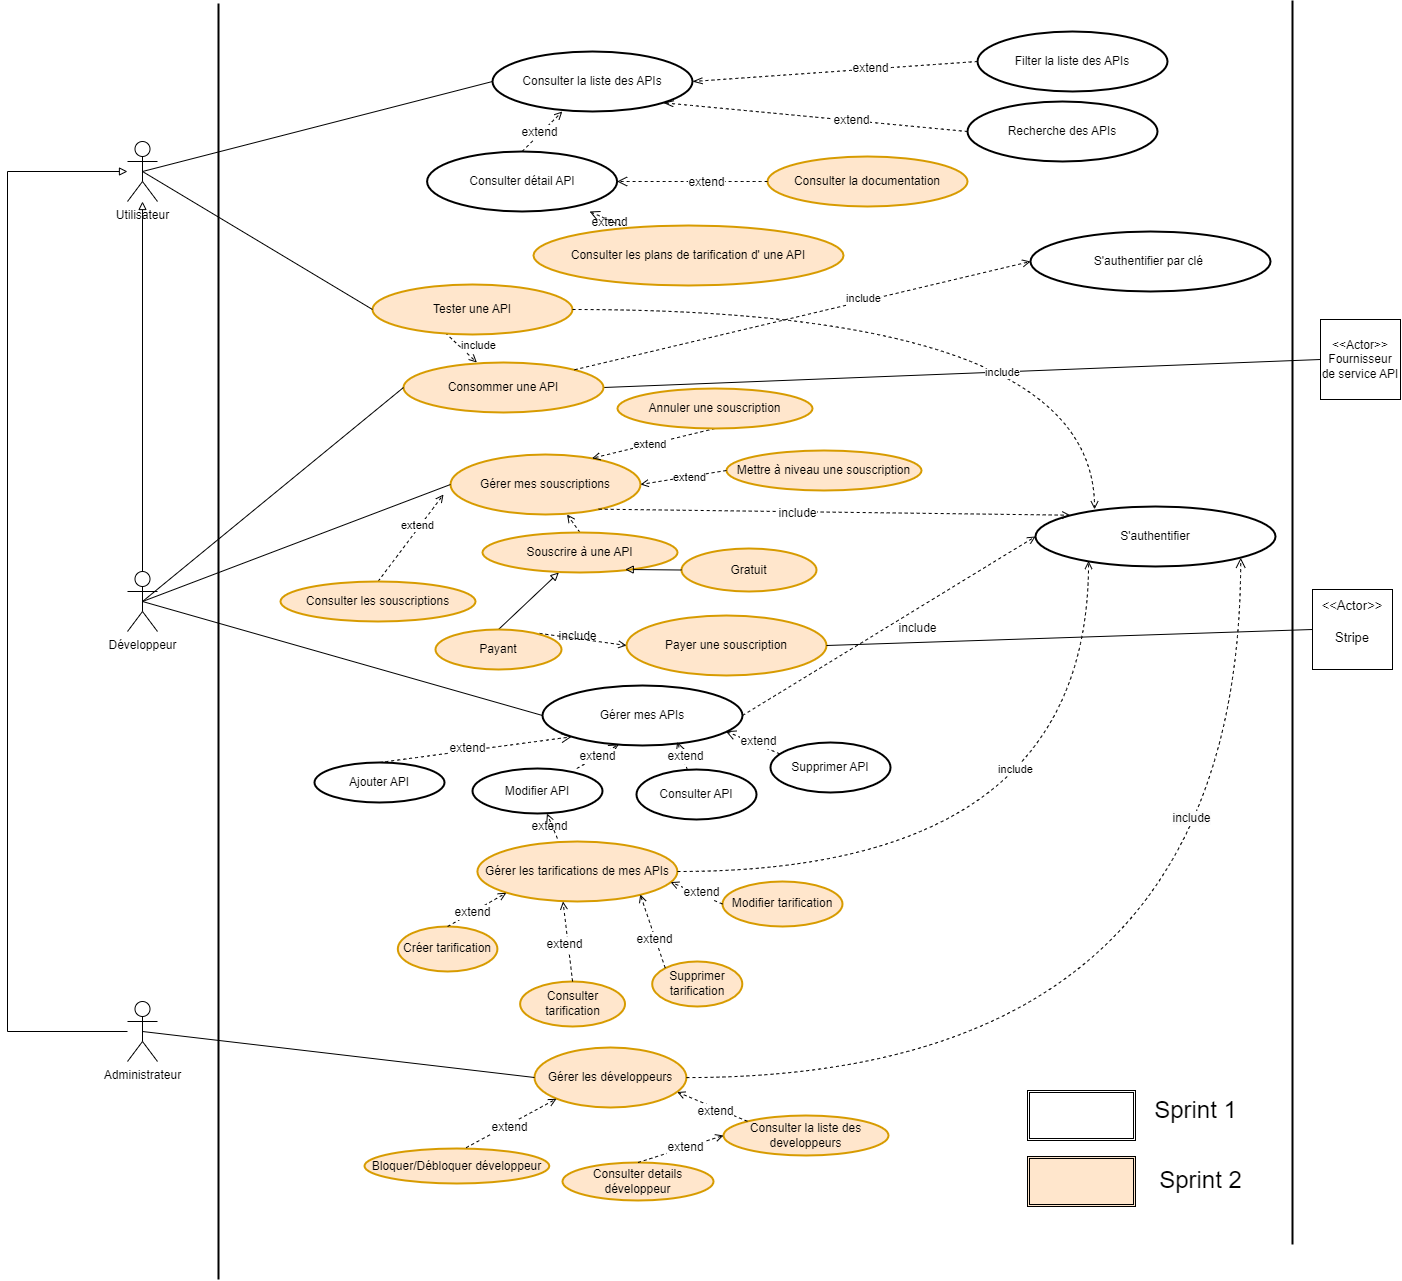
\includegraphics[width=1.1\columnwidth]{diagrammedecasdutilisationsprint2.png}}
    \caption{Diagramme de cas d'utilisation du sprint2}
    \label{fig:logo_tt}
\end{figure} 
\pagebreak

\subsection{Exemple d'une maquette d'interface du sprint 2 }
La figure suivante représente la maquette de l'interface d'ajout d'un plan de tarification dans la marketplace.
\begin{figure}[H]
    \centering
    \frame{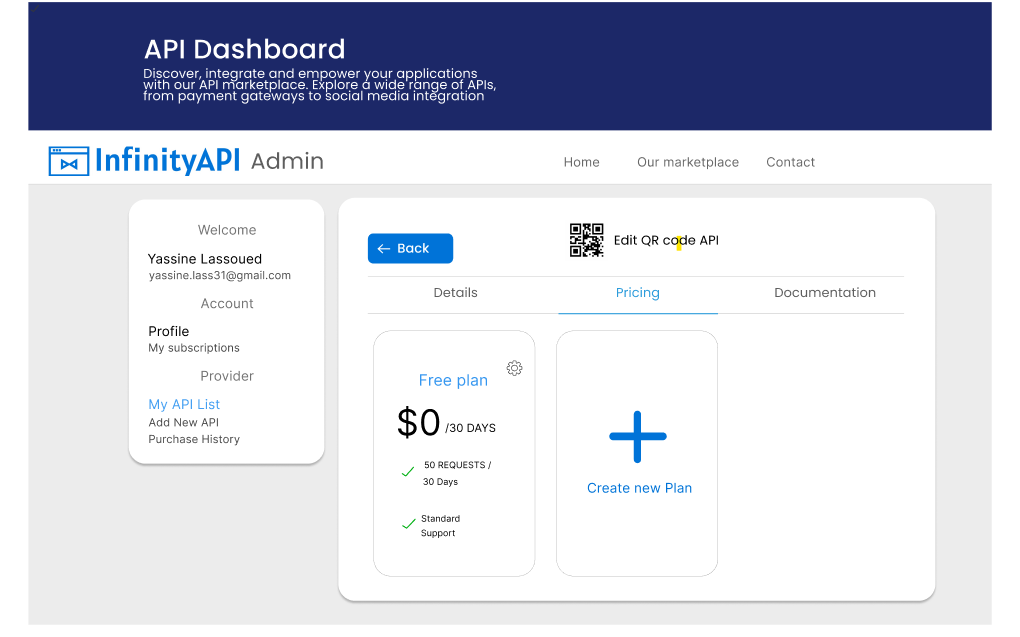
\includegraphics[width=1.1\columnwidth]{maquettetarificationAPI.png}}
    \caption{Maquette d'ajout d'un plan de tarification}
    \label{fig:logo_tt}
\end{figure}
\pagebreak

\section{Conception}
Dans cette partie, nous présentons le diagramme de classes, les diagrammes d'activités ainsi que les diagrammes de séquence afin d'illustrer les traitements des user stories clés de ce sprint, à savoir : l'ajout d'un plan de tarification, la souscription à une API et la consommation d'une API .
\subsection{Modélisation structurelle}

\subsubsection{Règles de gestion et de calcul}
Voici les principales règles de gestion avant de présenter le diagramme de classes :
\begin{itemize}
    \item  Une souscription peut être associée à zéro ou un paiement.
    \item Un paiement appartient à une seule souscription.
    \item Une souscription est effectuée pour un seul plan.
    \item Un plan peut être associé à zéro ou plusieurs souscriptions.
    \item Une requête est faite par un seul utilisateur.
    \item Un utilisateur peut déposer zéro ou plusieurs requêtes.
    \item Le pourcentage de commission de la plateforme est évalué à 15\%.
\end{itemize}

\subsubsection{Diagramme de classes}
\begin{figure}[H]
    \centering
    \frame{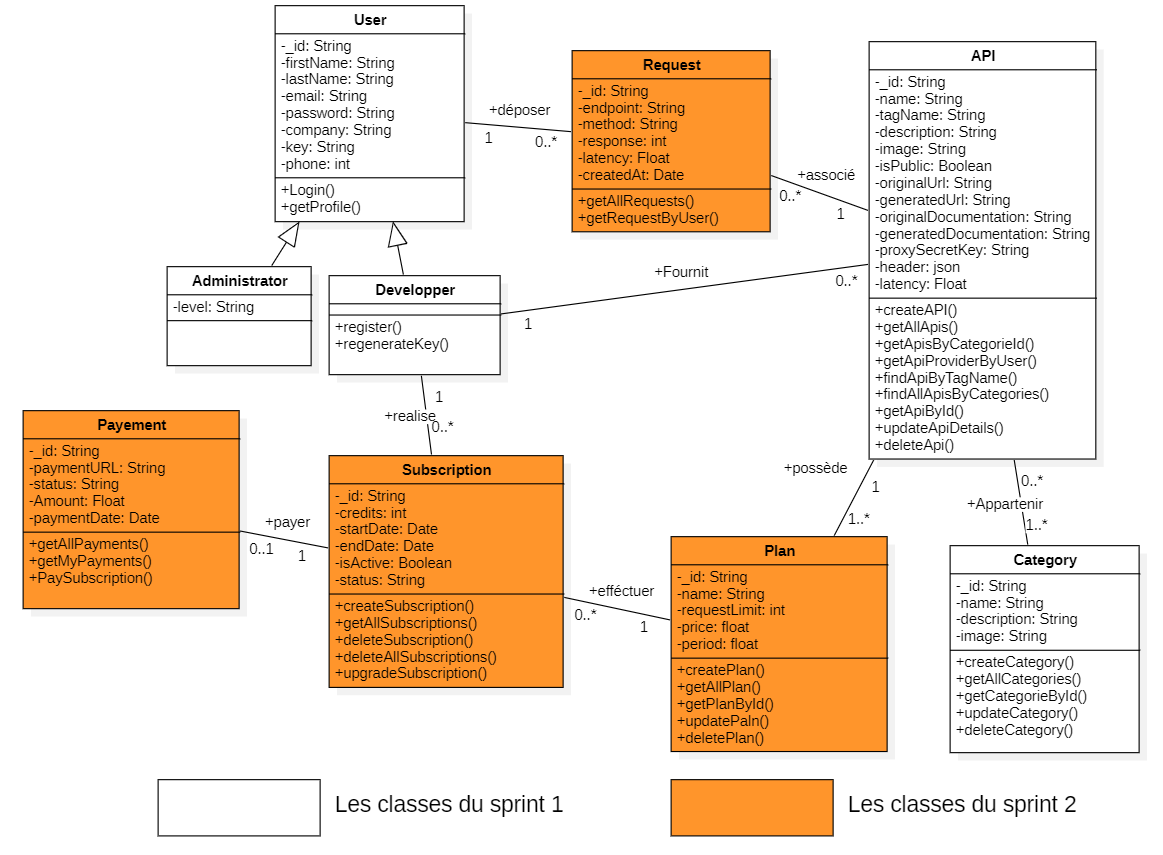
\includegraphics[width=0.8\columnwidth]{DiagrammeDeClasseDeSprint2.png}}
    \caption{Diagramme de classes du sprint 2}
    \label{fig:logo_tt}
\end{figure}
\pagebreak

\subsection{Diagramme d'activités "Ajouter un plan de tarification"}
Ce diagramme d'activités représente le processus de création d'un plan de tarification. Initialement, un développeur soumet les détails du plan via un formulaire. Ensuite, le système vérifie la validité du jeton JWT pour authentifier l'accès à l'API de tarification. \\
 Si le jeton est valide, le système procède à la vérification de l'existence de l'utilisateur. Si l'utilisateur n'existe pas, il est redirigé vers la page d'authentification. Sinon, le système vérifie si l'utilisateur est le fournisseur de l'API. \\
S'il est le fournisseur, le système vérifie l'unicité du nom  du plan ainsi que le prix .Si une quelconque condition n'est pas satisfaite, un message d'erreur est affiché. Sinon, le système vérifie si le nombre maximal de plans de tarification est dépassé. S'il est dépassé, une erreur est affichée. Une erreur sera également signalée si le nombre de requêtes ou la période correspondent déjà à un autre plan. Si aucune erreur n'est détectée, le plan est ajouté avec succès et un message de réussite est affiché.
\begin{figure}[H]
    \centering
    \frame{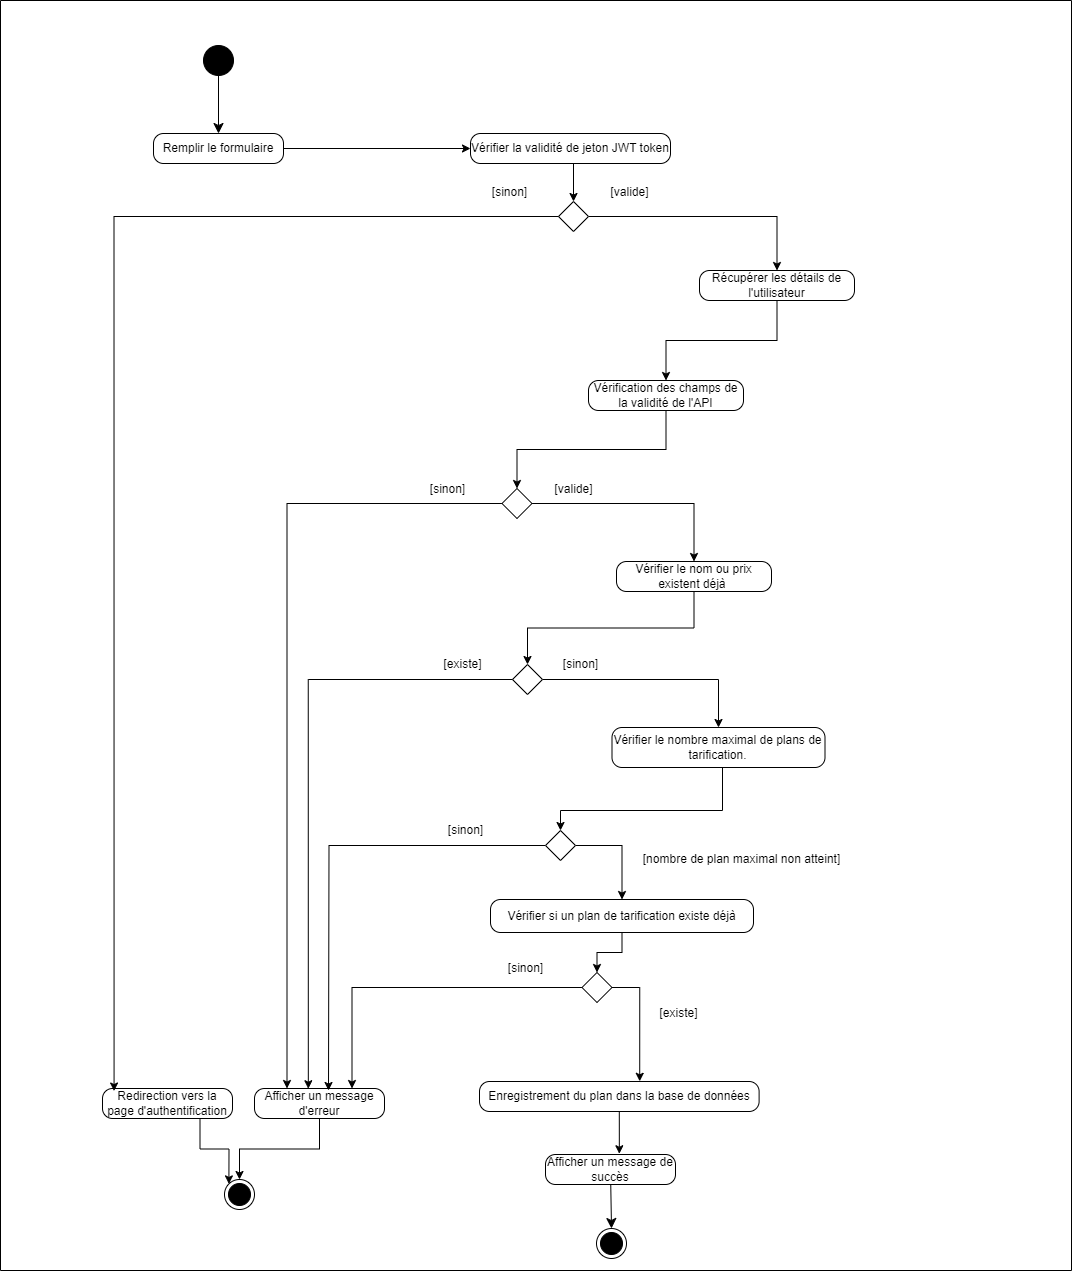
\includegraphics[width=1.1\columnwidth]{diagrammedactiviteAjouterPlandetarification.png}}
    \caption{Diagramme d'activités "Ajouter Plan de tarification"}
    \label{fig:logo_tt}
\end{figure}
\pagebreak

\subsection{Diagramme d'activités "Consommer une API "}
Ce diagramme d'activités décrit le processus de consommation d'une API. Tout commence lorsque le développeur envoie une demande de consommation. Le système vérifie d'abord la validité de la clé de l'utilisateur. Si elle est invalide, un message d'erreur est retourné. \\
Sinon, le système vérifie si l'API spécifiée existe. Si elle n'existe pas, un message d'erreur est retourné. Ensuite, la validité de la souscription est vérifiée. En cas de souscription invalide, une erreur est signalée. \\
Sinon, le système vérifie si l'endpoint spécifié existe. S'il n'existe pas, une erreur est retournée. Ensuite, le système crée une requête HTTP, y ajoute l’entête de  l'API, puis envoie la requête au fournisseur de services API. En cas de serveur hors service, un message d'erreur est affiché. \\
Si le serveur répond, le système enregistre la réponse et met à jour le crédit de l'utilisateur.
\begin{figure}[H]
    \centering
    \frame{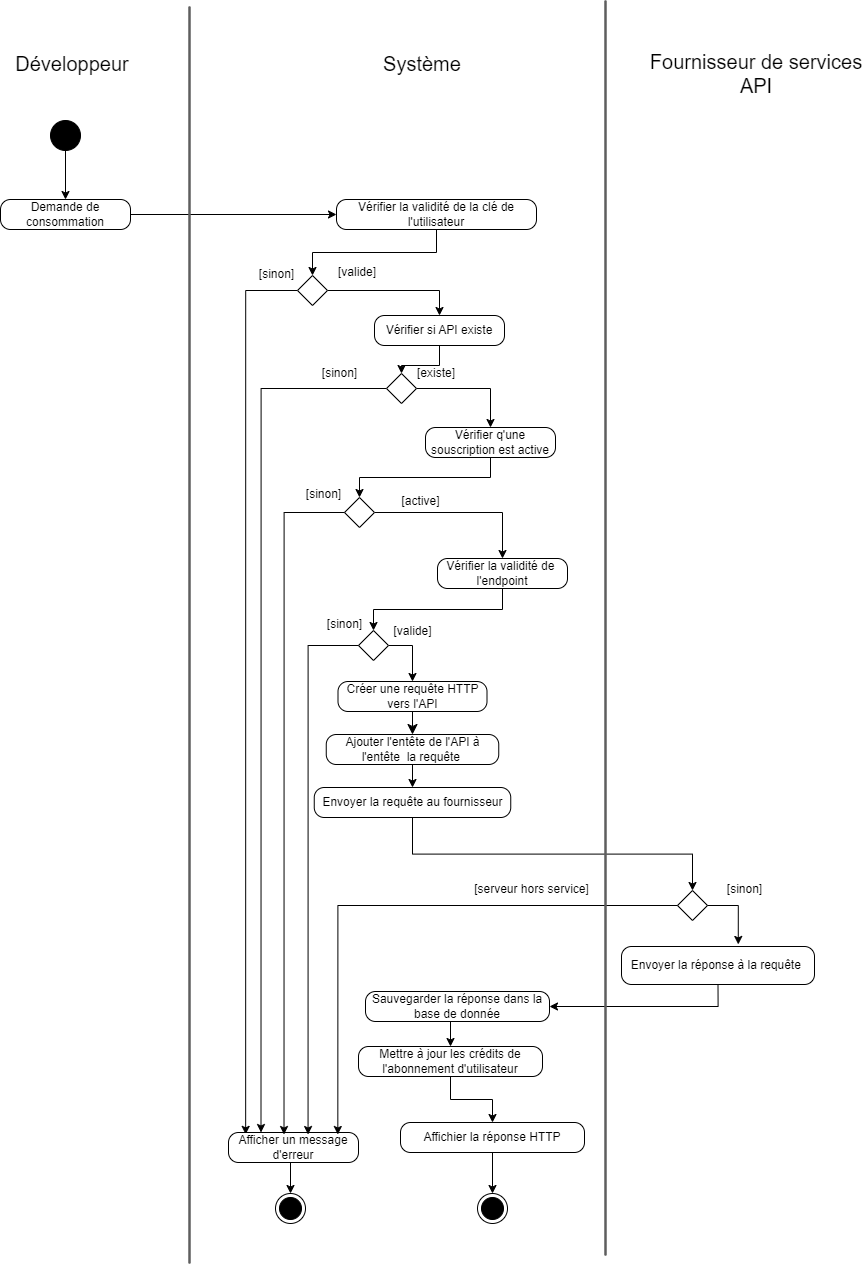
\includegraphics[width=1\columnwidth]{diagrammedactiviterconsommation.png}}
    \caption{Diagramme d'activités "Consommer une API "}
    \label{fig:logo_tt}
\end{figure}
\pagebreak

\subsection{Diagramme de séquence "Consommer une API"}
Ce diagramme de séquence illustre la séquence d'interactions entre les différents composants pour réaliser la consommation d’une API en dehors de la marketplace. Le processus commence lorsque le développeur exécute une requête. \\ 
Le middleware d'authentification vérifie si la clé existe dans la base de données. Si la clé n'existe pas, un message d’erreur est retourné. Sinon, le middleware API vérifie si l'API est valide. Si l'API est invalide, un message d’erreur est retourné. \\ 
Sinon, le middleware de souscription vérifie si la souscription est active. Si la souscription n'est pas valide, un message d'erreur est retourné .Sinon le contrôleur de consommation vérifie si le endpoint existe. S'il n'existe pas, un message d’erreur est retourné. \\
Sinon il  crée une requête HTTP, y ajoute l’en-tête de l'API, puis envoie la requête au fournisseur. La réponse est ensuite enregistrée au niveau de la classe request. En cas de serveur hors service, un message d'erreur est affiché. Sinon, le crédit de l'utilisateur est mis à jour et la réponse est affichée.
\begin{figure}[H]
    \centering
    \frame{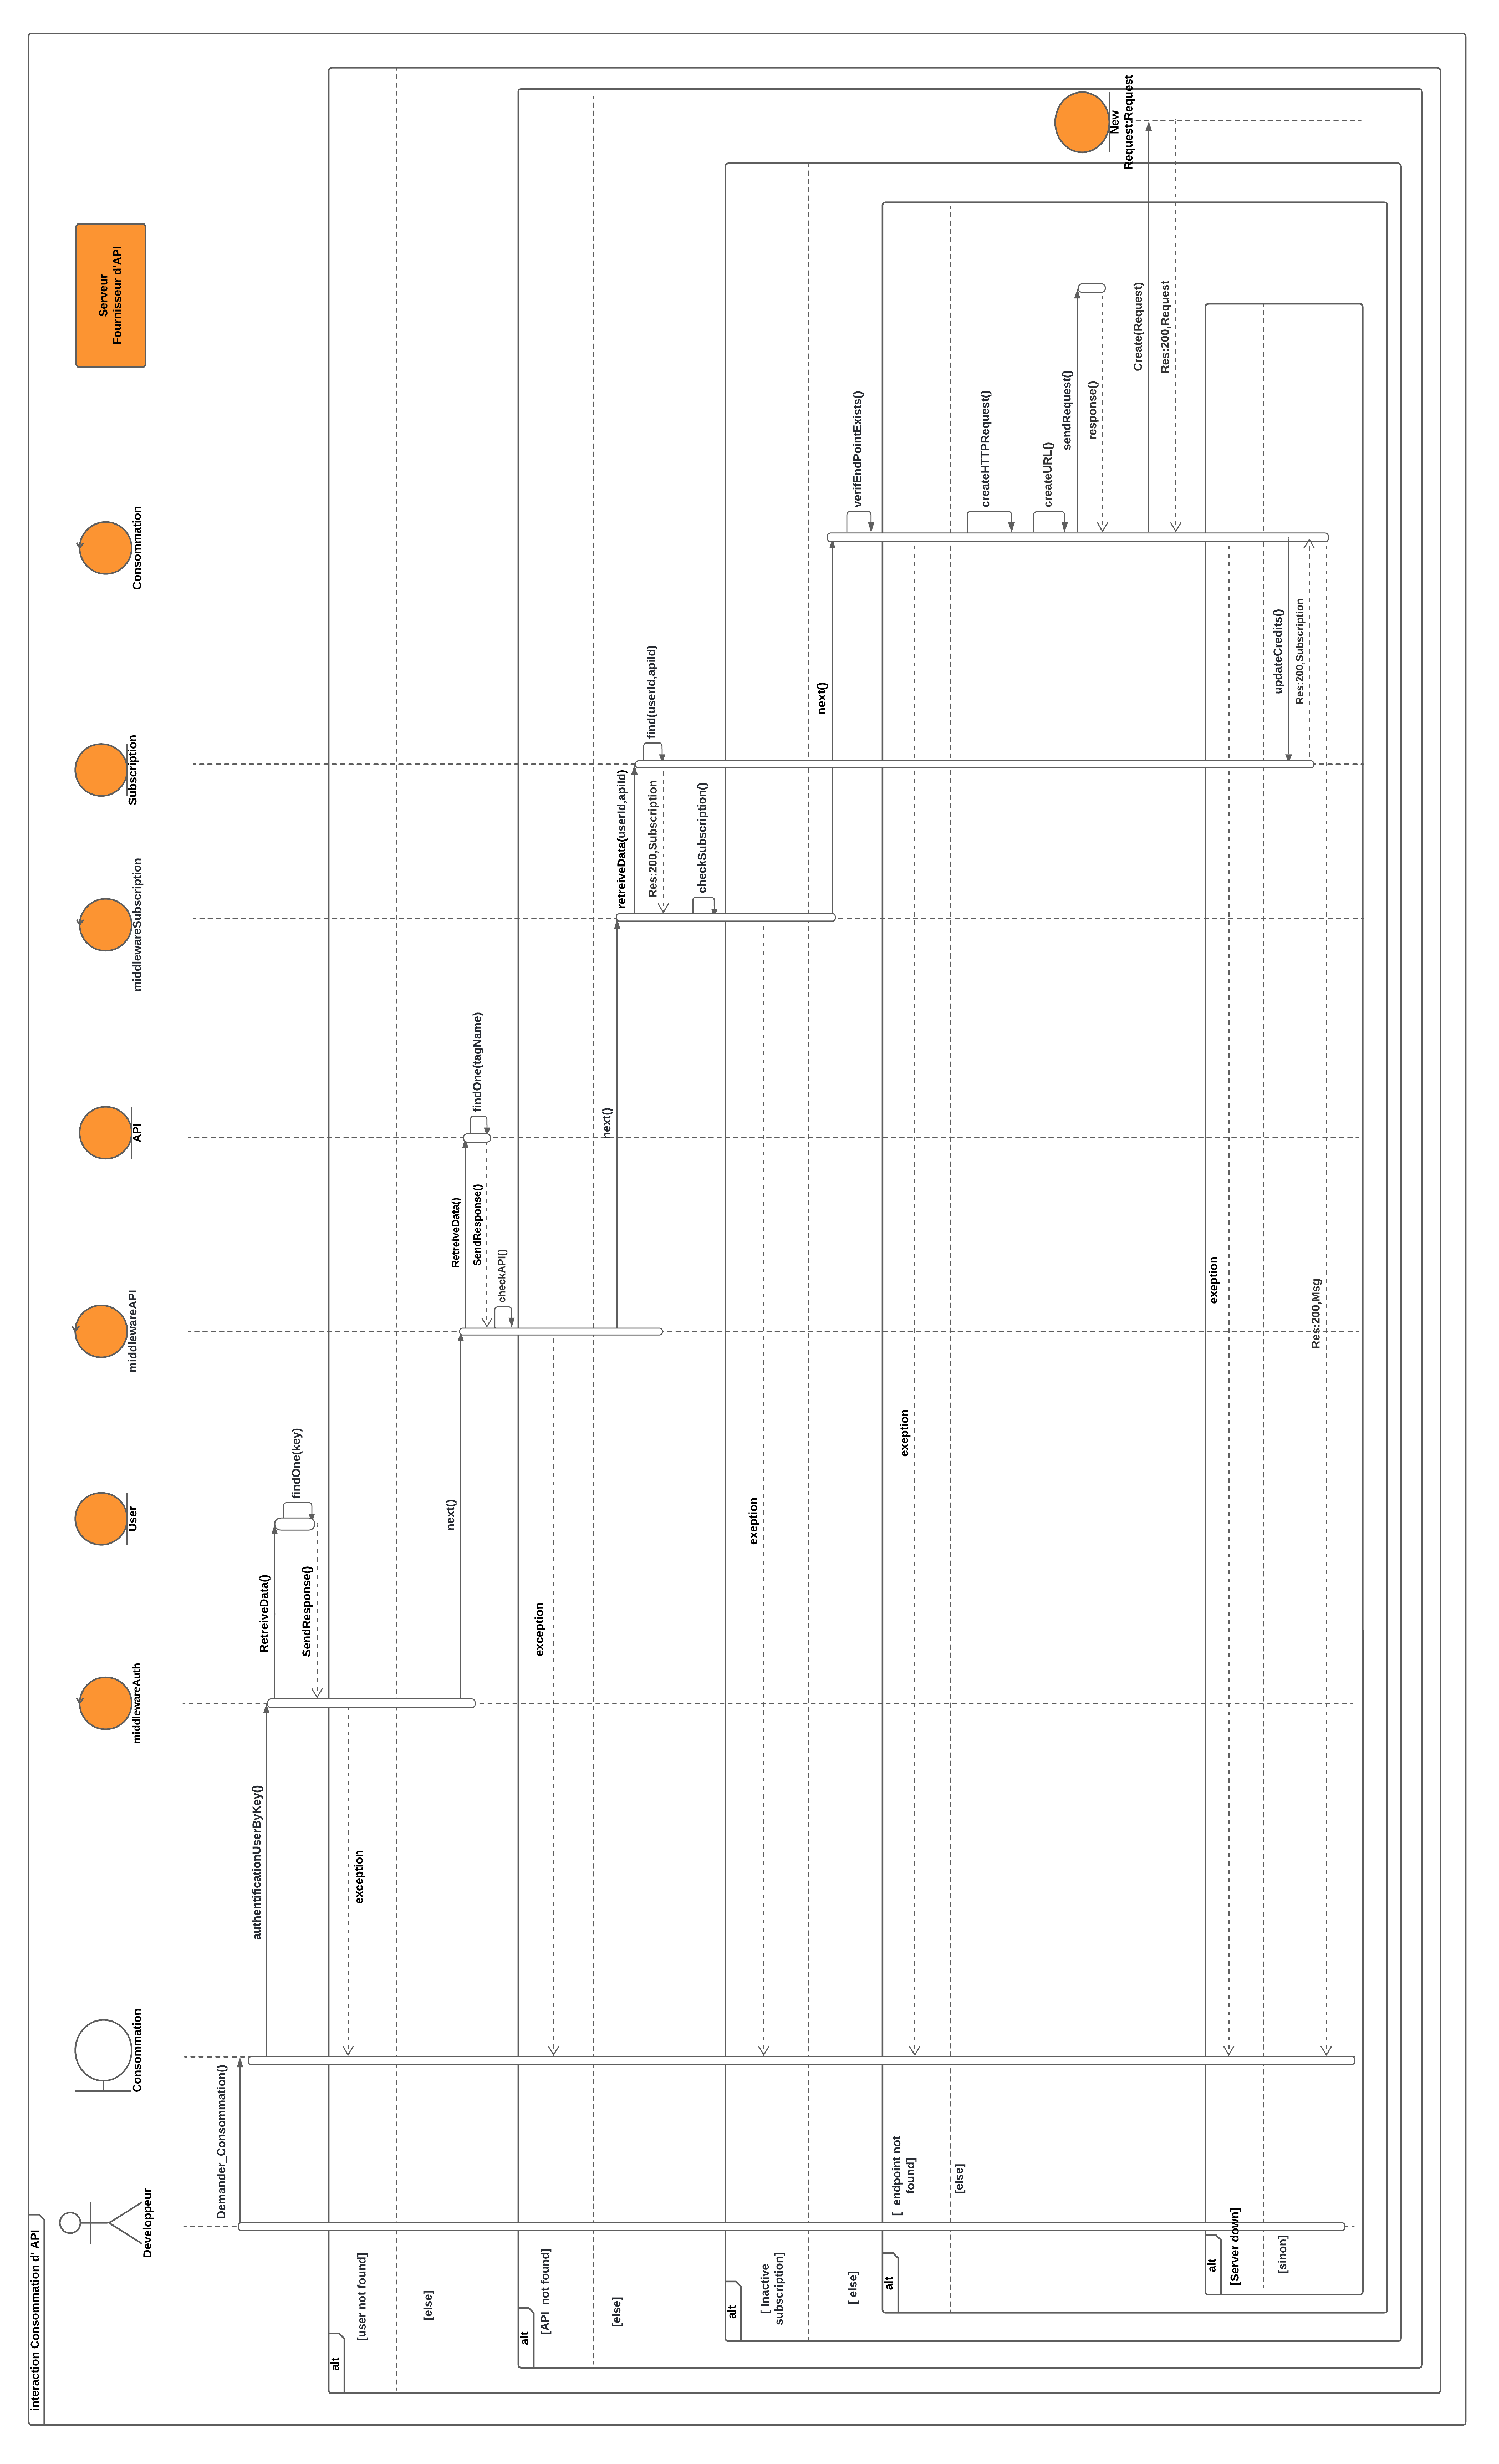
\includegraphics[width=0.9\columnwidth]{DiagrammeDeSequenceConsommation .png    }}
    \caption{Diagramme de séquence "Consommer une API"}
    \label{fig:logo_tt}
\end{figure}
\pagebreak

\subsection{Diagramme d'activités de "Souscription à une API"} 
Ce diagramme d’activités décrit le processus de souscription à une API. Tout commence lorsque le développeur envoie une demande de souscription. Le système vérifie d’abord la validité du jeton JWT. Si le jeton est invalide, un message d’erreur est retourné.  Sinon, le système récupère les détails de l'utilisateur et vérifie s'il possède déjà une souscription active. Si une souscription existe, un message d’erreur est retourné.\\
Ensuite, le système crée une nouvelle souscription. Si l'API est gratuite, la souscription est activée immédiatement et un message de succès est affiché. Si l'API est payante, le système crée un paiement en attente. \\
Stripe intervient alors pour créer une session de vérification de paiement et redirige vers l'URL de prise de la session. Stripe traite le paiement. En cas d'échec du paiement, il demande de réintroduire les données de paiement. Si le paiement est réussi, le système met à jour le statut de paiement, active la souscription et affiche un message de succès, puis redirige le développeur vers l'URL de succès. \\
\begin{figure}[H]
    \centering
    \frame{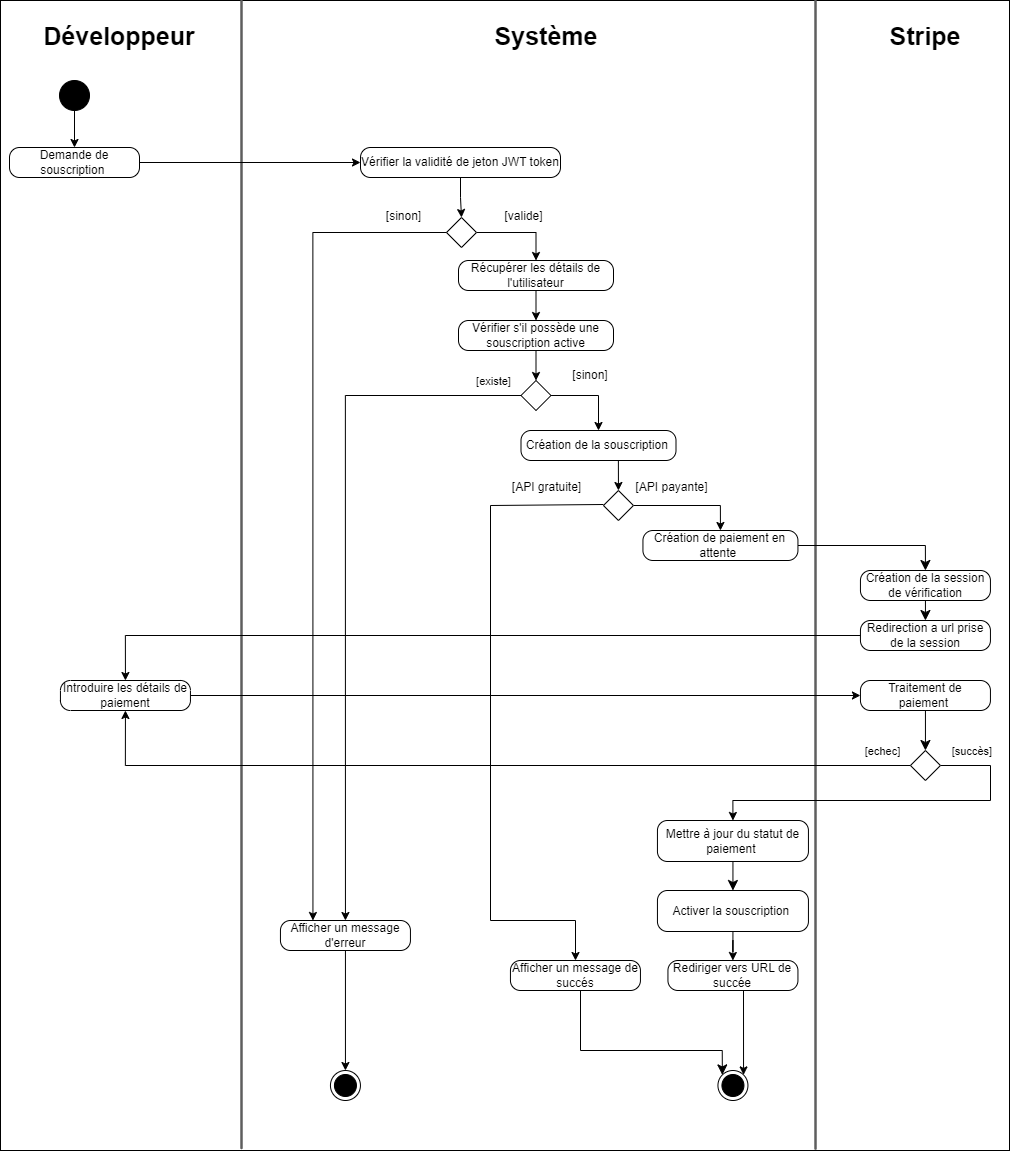
\includegraphics[width=1.1\columnwidth]{Diagrammedactivitedepaiement.png}}
    \caption{Diagramme d'activités "Souscription à une API" }
    \label{fig:logo_tt}
\end{figure}
\pagebreak

\section{Revue de sprint}
Dans cette partie, nous allons exposer le travail réalisé durant le sprint 2, ainsi que le burndown chart.
    \subsection{Réalisation}
    Dans cette étape, nous allons explorer les interfaces réalisées lors de ce sprint.
   
    \subsubsection{Gestion de la tarification}
    Cette interface représente le formulaire d'ajout d'un plan de tarification
    \begin{figure}[H]
        \centering
        \frame{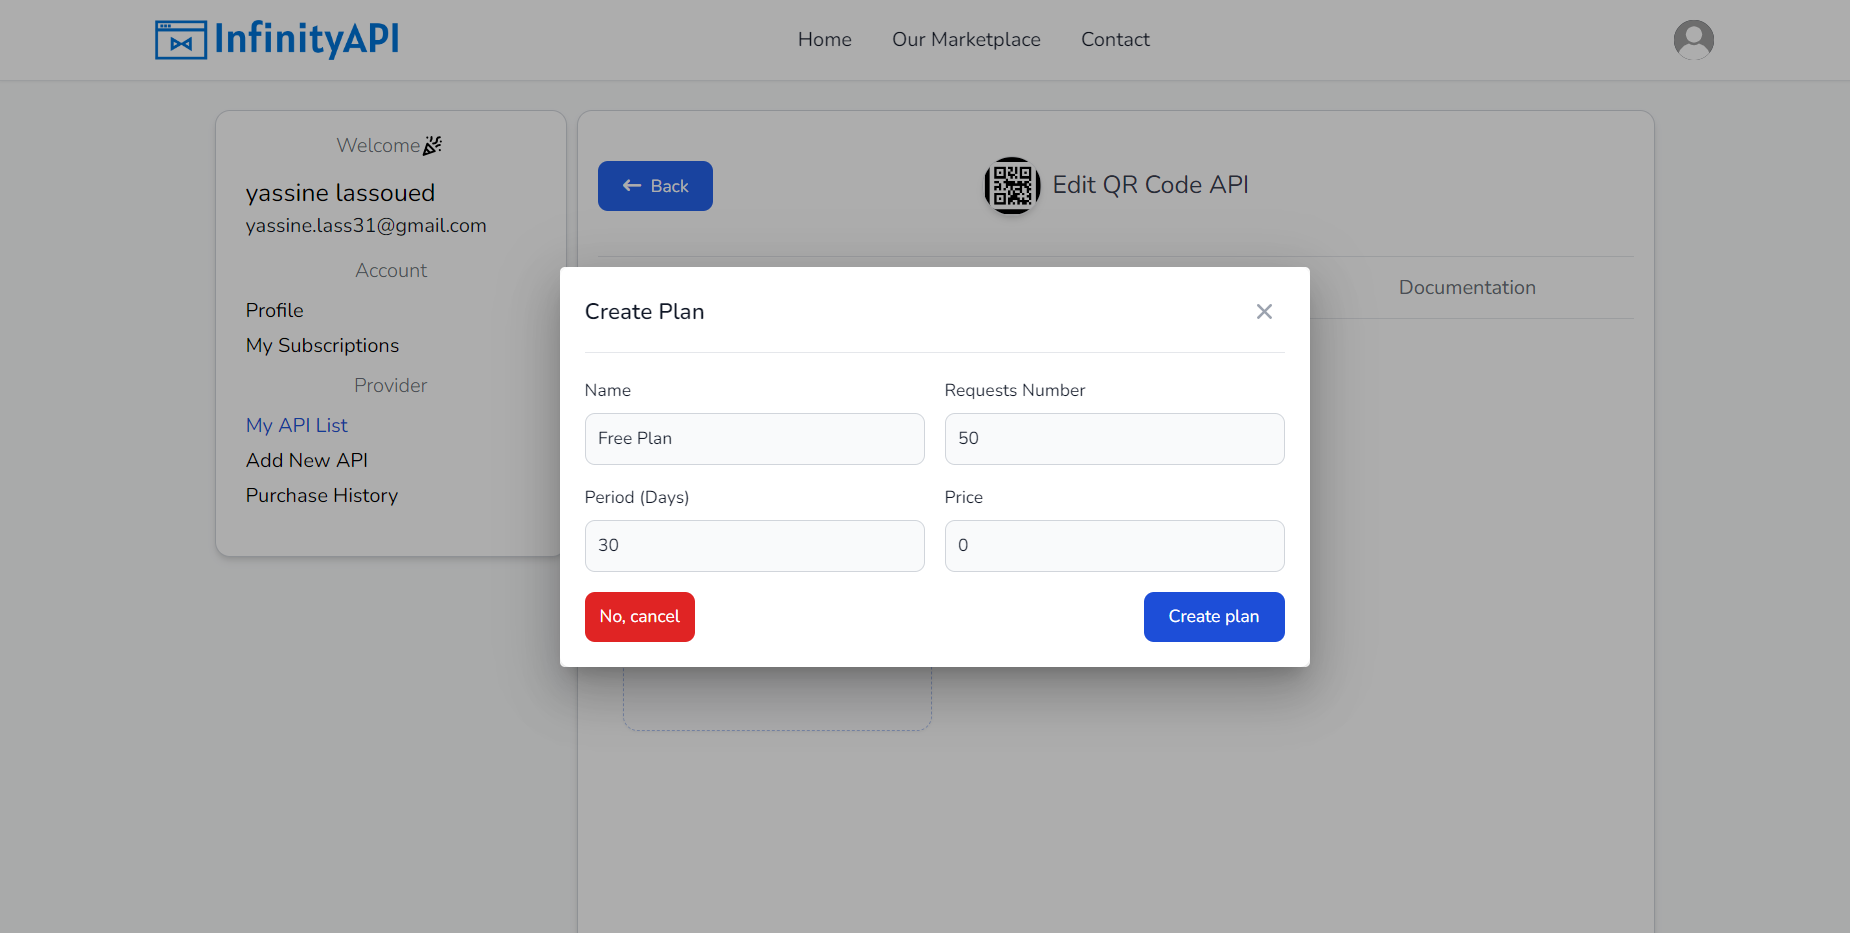
\includegraphics[width=0.7\columnwidth]{Interfacedajoutdeplandetarification.png}}
        \caption{ Interface d'ajout de plan de tarification }
        \label{fig:logo_tt}
    \end{figure}

    Après avoir rempli le formulaire, l'utilisateur peut consulter les plans de tarification ajoutés, et il peut cliquer sur "Créer un nouveau plan" à condition que le nombre de plans ne dépasse pas 4. 
    \begin{figure}[H]
        \centering
        \frame{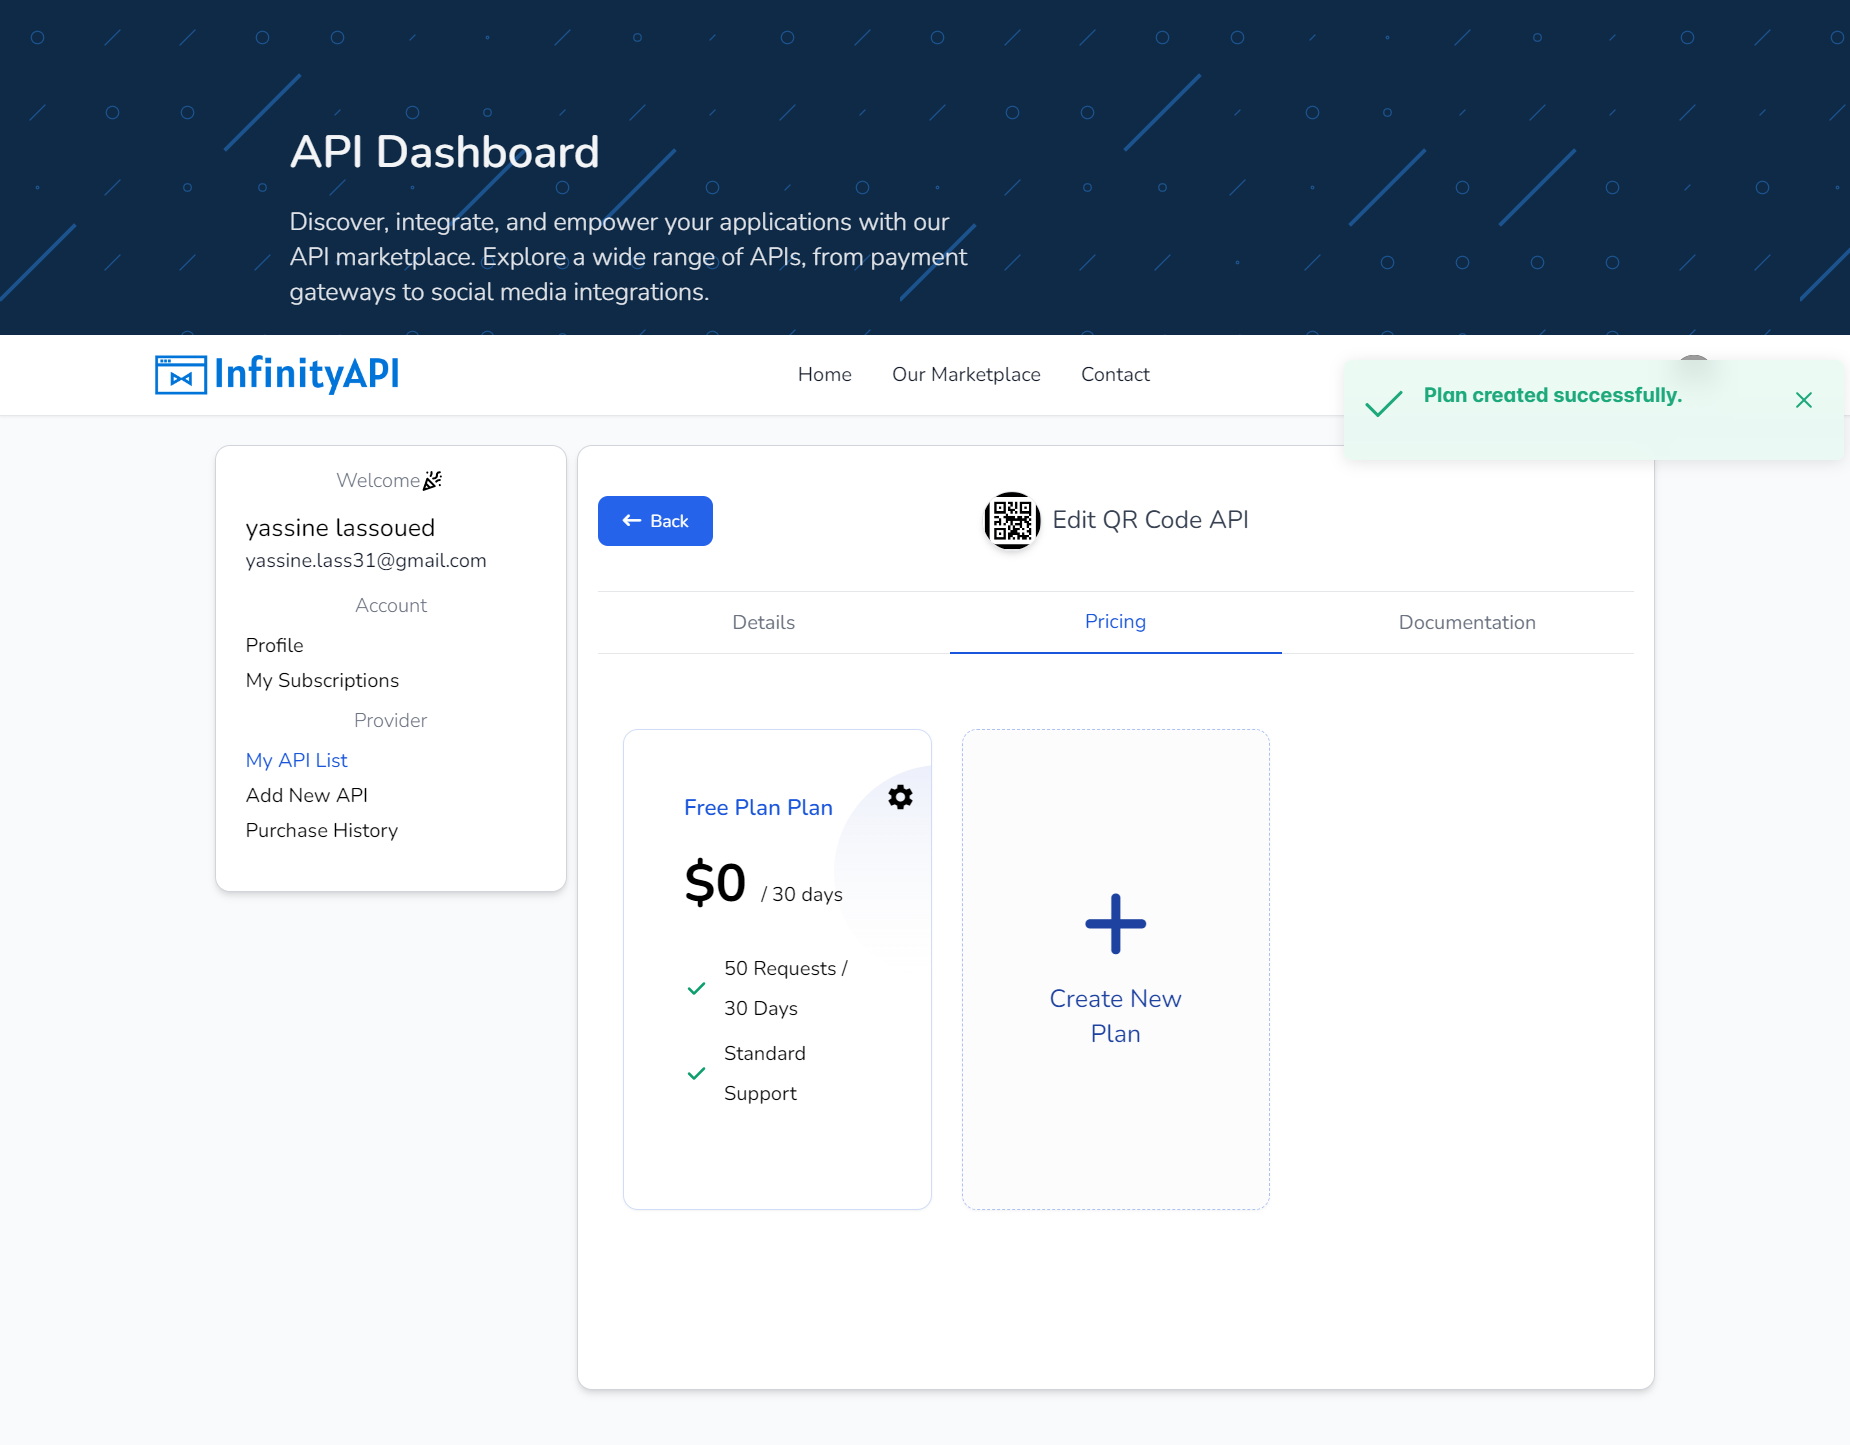
\includegraphics[width=0.6\columnwidth]{Interfacedelistedesplansdetarification.png}}
        \caption{ Interface de la liste des plans de tarification }
        \label{fig:logo_tt}
    \end{figure}

    \subsubsection{Souscription à une API }
    Cette interface représente le processus de souscription pour une API payante.
    \begin{figure}[H]
        \centering
        \frame{\includegraphics[width=1.1\columnwidth]{InterfacedeenchaînementdelasouscriptionauneAPI.png}}
        \caption{Interface de l'enchaînement de la souscription à une API }
        \label{fig:logo_tt}
    \end{figure}
    \pagebreak
    \subsubsection{Test d'API}
    Cette interface représente l'interface de test d'API dans notre plateforme.
    \begin{figure}[H]
        \centering
        \frame{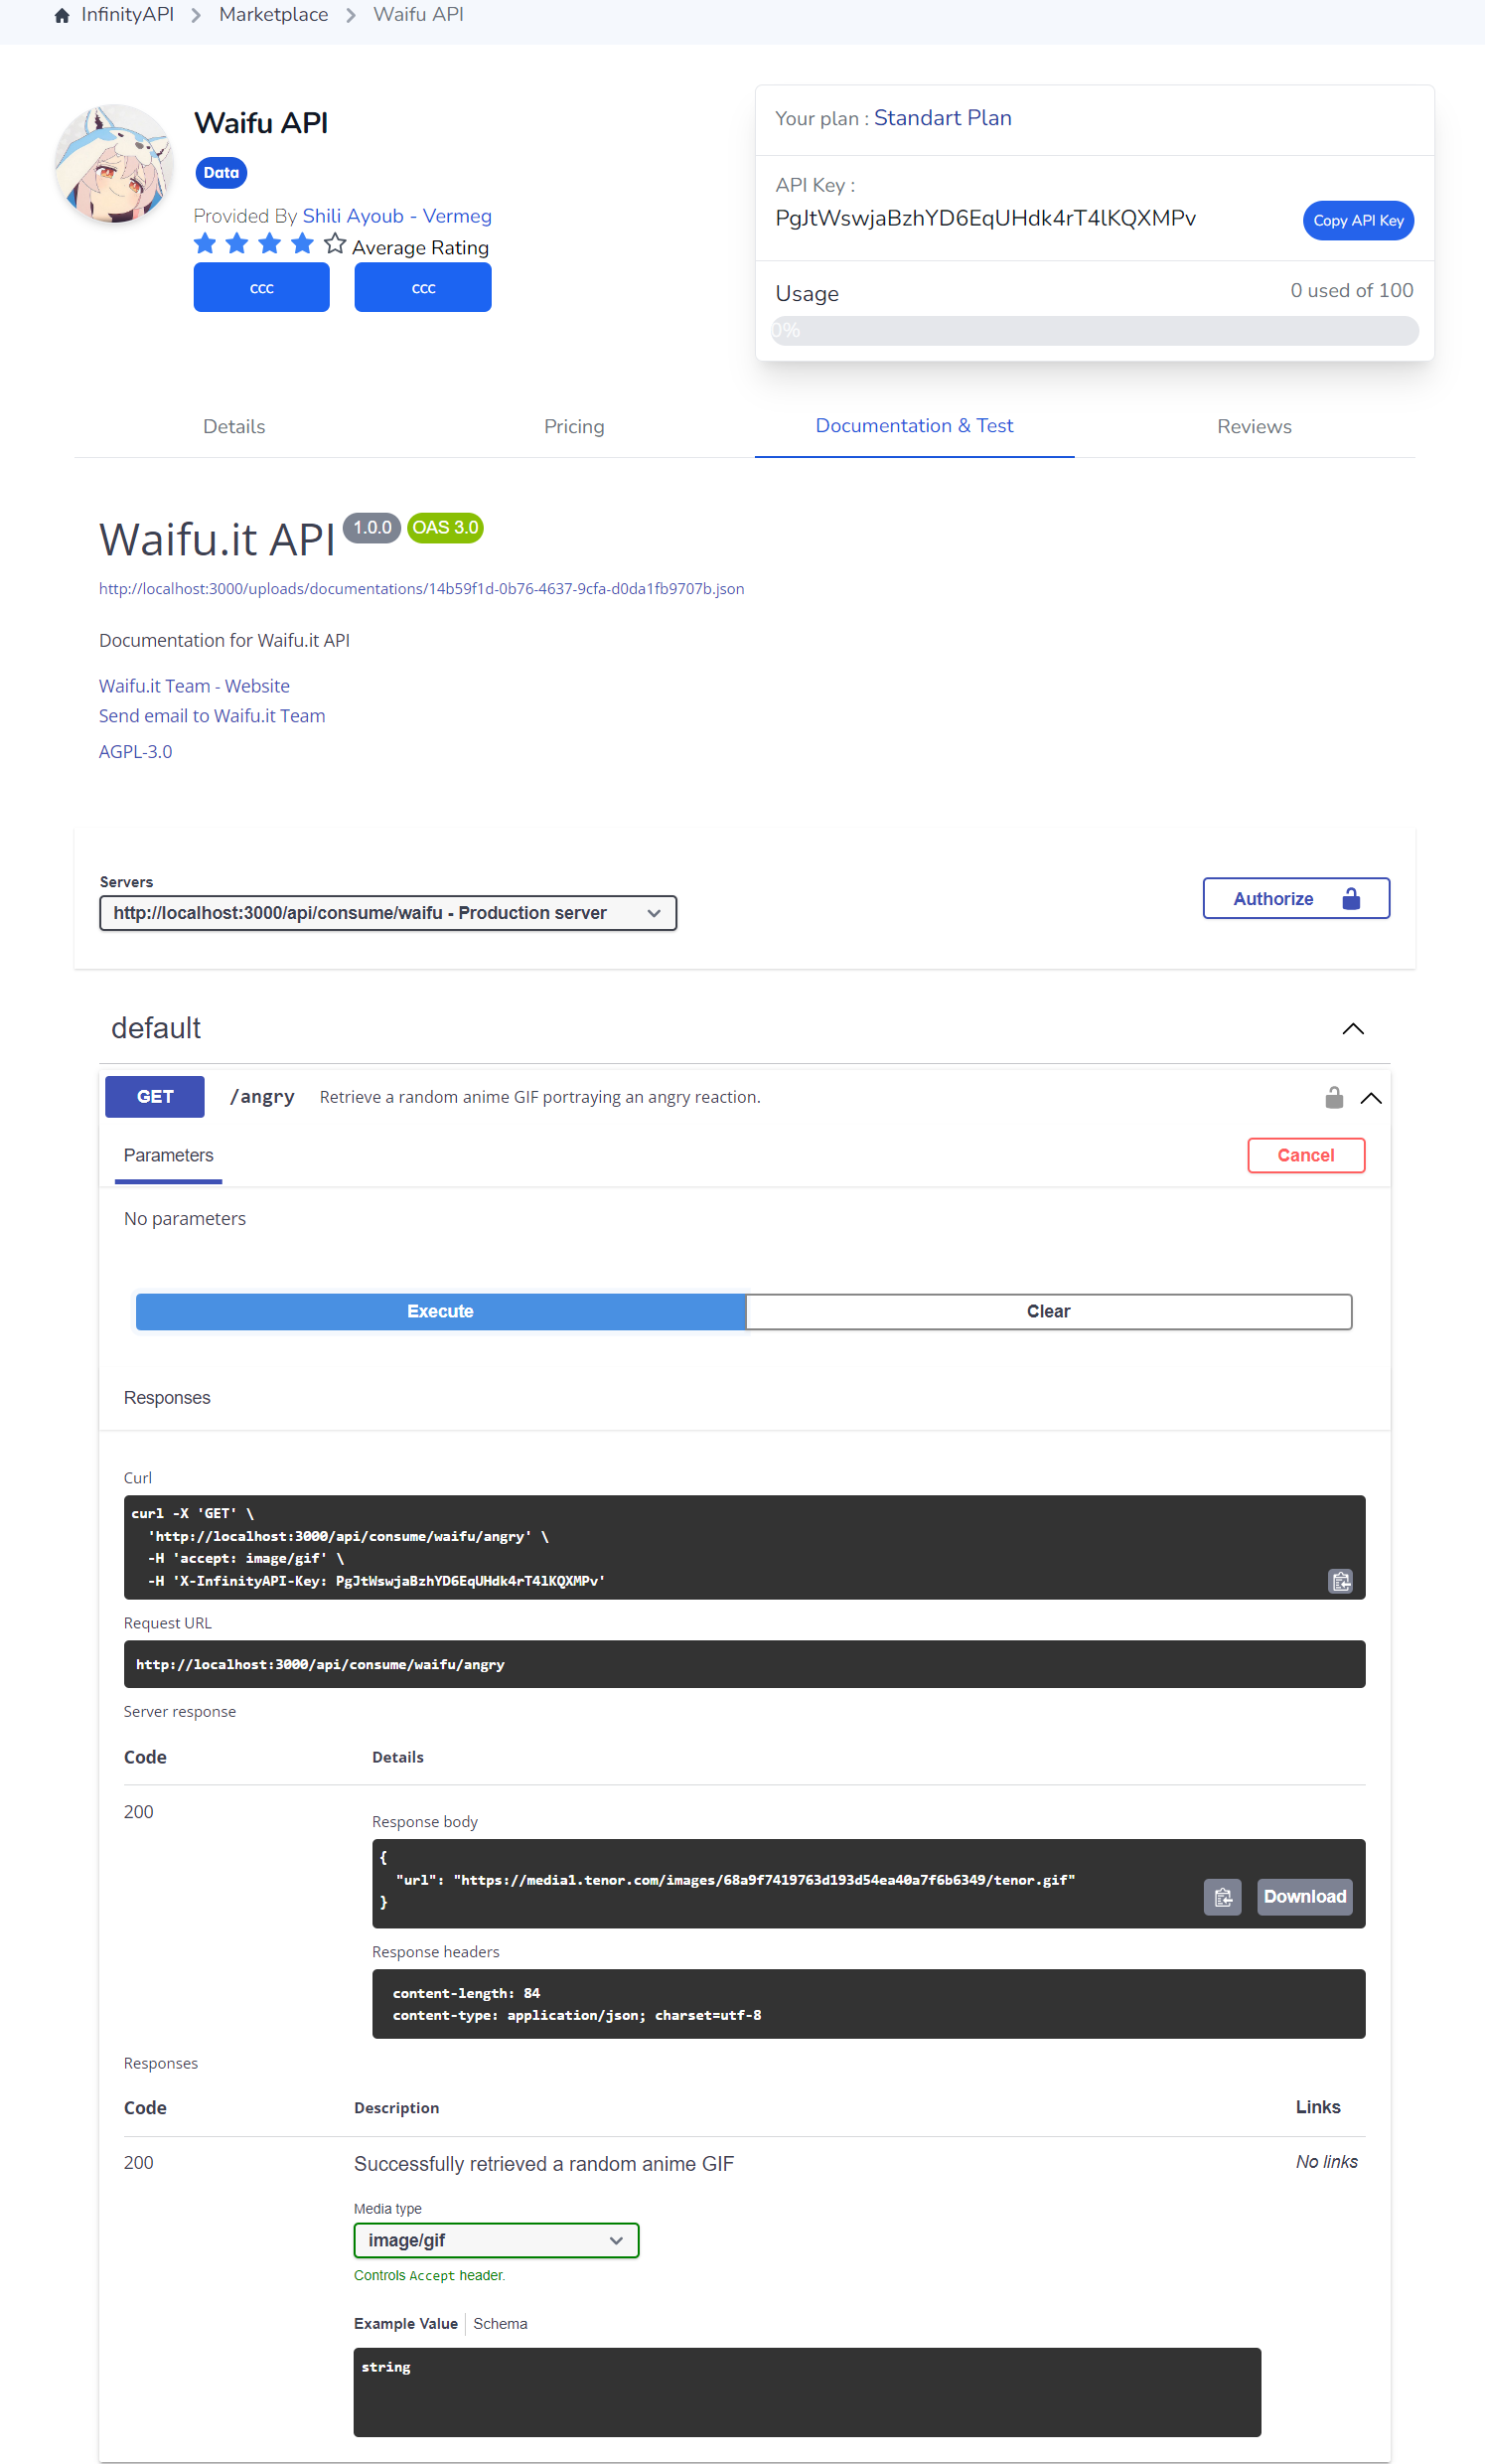
\includegraphics[width=0.8\columnwidth]{testAPI.png}}
        \caption{Interface de test d'une API}
        \label{fig:logo_tt}
    \end{figure}
    
    \subsubsection{Dashboard administrateur}
    Cette interface présente la liste des développeurs qui utilisent notre marketplace.       
        \begin{figure}[H]    
        \centering
            \frame{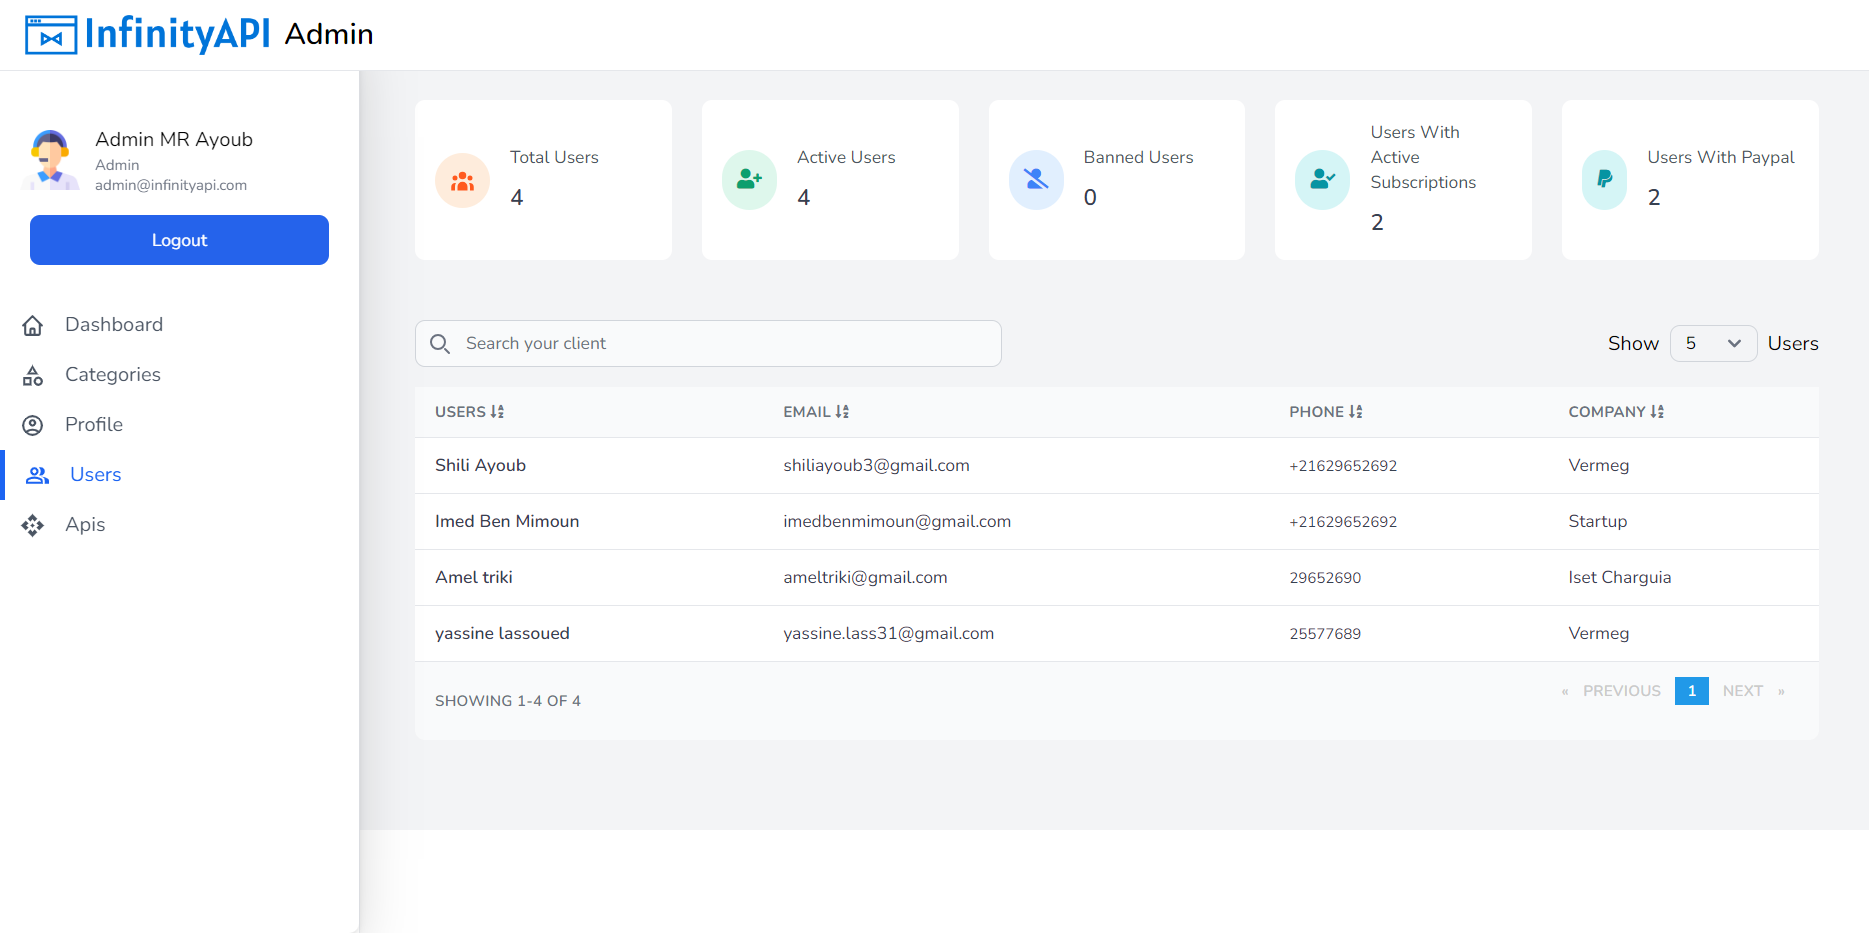
\includegraphics[width=1\columnwidth]{ListeUsers.png}}
            \caption{Interface de la liste des développeurs }
            \label{fig:logo_tt}
        \end{figure}

        Cette interface permet de gérer le profil d'un utilisateur, notamment en lui permettant de bloquer et de débloquer un utilisateur.
        \begin{figure}[H]    
        \centering
            \frame{\includegraphics[width=1\columnwidth]{ Interfacedeprofildéveloppeur.png     }}
            \caption{Interface de profil développeur }
            \label{fig:logo_tt}
        \end{figure}


        \subsection{Burndown Chart}
        \begin{figure}[H]    
            \centering
                \frame{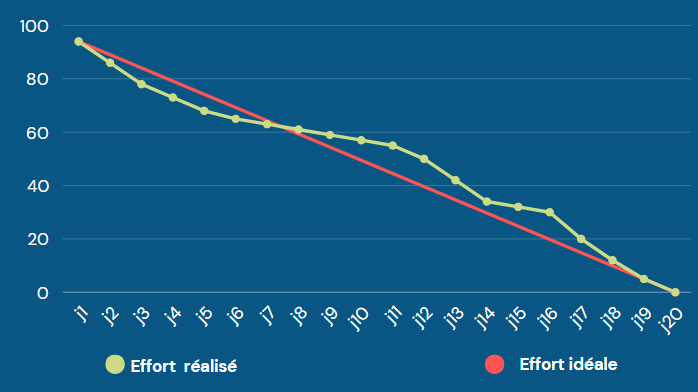
\includegraphics[width=0.9\columnwidth]{ Burndown_Chart_du_sprint2.png     }}
                \caption{Burndown chart du sprint 2}
                \label{fig:logo_tt}
            \end{figure} 
            Ce burndown montre que :
            \begin{itemize}
                \item Tous les user stories sont réalisés dans le temps estimé.
                \item La vélocité de notre équipe est 94
            \end{itemize}
            
            \subsection{Rétrospective du sprint 2}
            \begin{longtable}[c]{|p{0.25\linewidth}|p{0.7\linewidth}|}
                \hline
                \textbf{Les questions} & \textbf{Les réponses} \\
                \hline
                \endfirsthead
                \multicolumn{2}{c}%
                {{\bfseries \tablename\ \thetable{} -- suite de la page précédente}} \\
                \hline
                \textbf{Les questions} & \textbf{Les réponses} \\
                \hline
                \endhead
                \hline \multicolumn{2}{|r|}{{\bfseries Suite à la page suivante}} \\
                \hline
                \endfoot
                \hline
                \endlastfoot
            
                \multirow{3}{=}{Ce qui s'est bien passé} & Maîtrise de l'intégration de l'API Stripe \\
                & Avancement des fonctionnalités clés\\
                &Collaboration efficace \\
                \hline
                \multirow{2}{=}{Les problèmes rencontrés} & Déséquilibre dans le temps de travail pendant le mois de Ramadan \\
                & Problèmes d'intégration\\
                \hline
                \multirow{1}{=}{Les choses à améliorer} &Tests plus rigoureux \\
                \hline
            \end{longtable}

\section*{Conclusion}
Tout au long de ce chapitre, nous avons présenté le travail effectué au niveau du deuxième sprint, en termes de spécification, conception et réalisation. Dans le chapitre suivant, nous aborderons le dernier sprint.